% D.28 直角三角形内切圆 & 外接圆，直角边 6、8
\documentclass[tikz,border=4pt]{standalone}
\usepackage{ctex}
\usepackage{amsmath}
\usetikzlibrary{calc}
\begin{document}
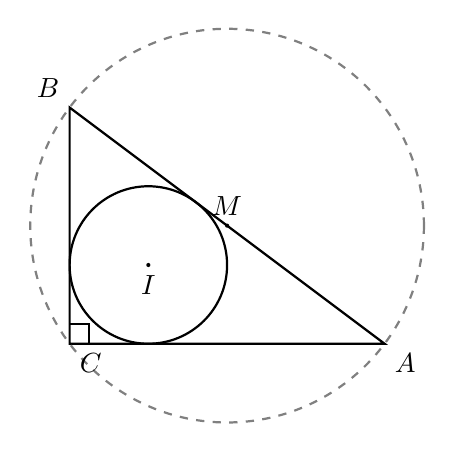
\begin{tikzpicture}[scale=0.5, thick]
  \coordinate (C) at (0, 0);
  \coordinate (A) at (8, 0);
  \coordinate (B) at (0, 6);
  \pgfmathsetmacro{\rin}{2}    % r = (a+b-c)/2 = (6+8-10)/2 = 2
  \pgfmathsetmacro{\rout}{5}   % R = c/2 = 5
  \coordinate (I) at (2, 2);
  \coordinate (M) at (4, 3);   % 斜边中点

  \draw (A) -- (B) -- (C) -- cycle;
  \draw (I) circle (\rin);
  \draw[gray, dashed] (M) circle (\rout);

  \draw (0.5, 0) -- (0.5, 0.5) -- (0, 0.5);

  \fill (I) circle (1.5pt);
  \fill (M) circle (1.5pt);
  \node[below right] at (C) {$C$};
  \node[below right] at (A) {$A$};
  \node[above left]  at (B) {$B$};
  \node[below]       at (I) {$I$};
  \node[above]       at (M) {$M$};
\end{tikzpicture}
\end{document}
